% =========================================================================
% How Much of a Convolutional Layer's Width Is Actually Used?
%
% First complete draft (tag v0.1-first-full-draft, 2026-09-15); revised
% 2026-09-16 after the hostile-review exercise (notes/hostile-review-2026-09-15.md).
% \todo{...} marks text that cannot be written before submission.
%
% The analysis plan lives at ../notes/analysis-plan.md.  If this document and
% that one disagree, the plan wins and this file is out of date.
% Verification notes for three contested references: ../refs/verification-notes.md
%
% Build:  make tectonic ; make supp      Outstanding items:  make todo
% =========================================================================

\documentclass[10pt,journal,compsoc]{IEEEtran}

\usepackage{amsmath,amssymb,amsthm}
\newtheorem{proposition}{Proposition}
\newtheorem{corollary}{Corollary}
\usepackage{graphicx}
\usepackage{booktabs}
\usepackage{array}
\usepackage{url}
\usepackage[caption=false,font=footnotesize]{subfig}
\usepackage[hidelinks]{hyperref}
% IEEEtran compsoc sets Palatino (ppl); under XeTeX/tectonic load its metric clone so page counts match the CS template
\usepackage{iftex}
\ifXeTeX\usepackage{fontspec}\setmainfont{texgyrepagella}[Extension=.otf,UprightFont=*-regular,BoldFont=*-bold,ItalicFont=*-italic,BoldItalicFont=*-bolditalic]\fi

\graphicspath{{../results/figures/}}

% --- drafting aids; delete before submission ------------------------------
\usepackage{xcolor}
\newcommand{\todo}[1]{\textcolor{red}{[\textbf{TODO} #1]}}
% -------------------------------------------------------------------------

\begin{document}

\title{Measuring the Effective Width of Convolutional Layers: Protocol, Pitfalls, and the Comparison with Initialisation}

\author{Cheng-Chung~Li%
\IEEEcompsocitemizethanks{\IEEEcompsocthanksitem C.-C. Li is with the Taiwan Power
Research Institute, Taiwan Power Company, Taipei, Taiwan.\protect\\
E-mail: u324057@taipower.com.tw}%
}

\markboth{IEEE Transactions on Pattern Analysis and Machine Intelligence}%
{Li: Measuring the Effective Width of Convolutional Layers}

\IEEEtitleabstractindextext{%
\begin{abstract}
How much of a convolutional layer's channel width does a trained network
use? Two published depth profiles of this quantity disagree. We show that
they measure different objects, set by three choices made without
comment: the denominator, the covariance estimator and the tensor read.
Each moves a profile by more than the effects reported. The nominal width
overstates a $1\!\times\!1$ expansion layer's attainable rank by its
expansion ratio; global pooling lowers a profile by about twice its own
layer-to-layer step; the block output exceeds the rank bound of its last
convolution by the expansion ratio. The resulting protocol recovers the
CIFAR-10 profile of Garg \emph{et al.} ($r = 0.98$) and the ImageNet
values of Elmoznino and Bonner at every block that passes its sample-size
gate. Because the pre-activation covariance is exactly
$W\Sigma_{\rm patch}W^{\top}$, the width separates into an architectural,
a data and a kernel factor. On 44 checkpoints of eleven families measured
against their own initialisations, most families keep the ordering their
architecture gave them and gain a level; on ten of them the decomposition
shows training moving the bottleneck from the data to the kernel, whose
gain aligns with its input's principal directions. Read after the
nonlinearity, the widths can be trained to: a VGG-16 built at them
matches full width on CIFAR-10 at two thirds of the parameters, and a
pre-registered control ties that margin to the few-class task. Orthogonality penalties realise half of the width
gain the decomposition predicts. Code, spectra and the pre-registered
plan are released.
\end{abstract}

\begin{IEEEkeywords}
Convolutional networks, effective dimensionality, channel covariance,
network width, representation analysis.
\end{IEEEkeywords}}

\maketitle

% =========================================================================
\IEEEdisplaynontitleabstractindextext
\IEEEpeerreviewmaketitle


% =========================================================================
\IEEEraisesectionheading{\section{Introduction}\label{sec:intro}}

\IEEEPARstart{T}{he} number of channels in a convolutional layer is fixed
before training, and how many of them the trained layer uses is known,
if at all, only afterwards \cite{garg2019lowEffort,elmoznino2024highDim}.
Theory bounds the number without locating it: the infinite-width limit
describes the regime in which no feature is learned
\cite{jacot2018ntk,lee2020wide}, minimum-width theorems say what a family
\emph{can} represent \cite{park2021minimum}, and rank bounds bracket a
layer from above \cite{han2021rexnet,kim2018rank1} and below
\cite{daneshmand2020bn}. Every usable number is post hoc, and the post-hoc
numbers disagree: Garg \emph{et al.} \cite{garg2019lowEffort}, counting the
principal components of the channel covariance that reach $99.9\%$ of the
variance on CIFAR VGGs, report a profile that saturates mid-network and
collapses in its last layers; Elmoznino and Bonner
\cite{elmoznino2024highDim}, with the participation ratio over
568 ImageNet layers, report it rising with depth.

Setting out to reconcile the two, we found that the measurements differ
in three choices made without comment, each of which moves a profile by
more than the effects either paper reports: what the count is divided by,
whether spatial positions or pooled images are the observations, and
whether the convolution output or the block output is read. A
$1\!\times\!1$ expansion from $C_{\rm in}$ to $C_{\rm out} > C_{\rm in}$
channels cannot have output rank above $C_{\rm in}$, a bound stated before
\cite{han2021rexnet,kim2018rank1} but never carried into a profile; 20 of
ResNet-50's 53 convolutions are such layers, and a profile divided by
nominal width reads them as a tenth used whatever they have learned.

In this paper we fix a protocol in which each choice is explicit and its
consequence quantified, built on one identity: before its nonlinearity, a
convolution's output covariance is exactly $W\Sigma_{\rm patch}W^{\top}$.
The identity splits the effective width of a layer into what the
architecture permits, the attainable rank $r_{\max}$; what the data
supplies, $\Sigma_{\rm patch}$; and what learning does, the alignment of
$W$ with $\Sigma_{\rm patch}$; each factor is pinned by an identity and a
measurement. We validate the protocol against both published
estimators at both tensors, measure 19 public ImageNet checkpoints and
then 44 trained checkpoints of eleven families against their own
initialisations under a pre-registered plan, and put the ruler to use.

\subsection{Related Work}
\label{sec:related}

\textbf{What is measured.}\label{sec:four} Everything here is a functional of
the channel-covariance spectrum at one tensor, not a manifold intrinsic
dimension; the two differ by an order of magnitude on the same VGG-16
layer (TwoNN 18 against 200 principal components at $90\%$
variance \cite{ansuini2019intrinsic}). It is the linear count that width
concerns, because the consumer of a layer's output is the next
convolution, linear in its input patch; Section~\ref{sec:projection} makes
that operational.

\textbf{Depth profiles of dimensionality.}\label{sec:profiles} The
reported shape follows the measure: manifold dimension rises then falls
\cite{ansuini2019intrinsic}, the pooled participation ratio rises
\cite{elmoznino2024highDim}, the position-sampled $k^*$ saturates and
collapses on CIFAR \cite{garg2019lowEffort}, and the numerical rank of
deep layers falls to about the class count on CIFAR within a few hundred
steps \cite{masarczyk2023tunnel}, as neural collapse predicts for the
penultimate layer \cite{papyan2020neuralCollapse}, and the numerical rank
of the network's Jacobian falls monotonically with depth
\cite{feng2022rankDiminishing}. The bound $r_{\max}$
of Section~\ref{sec:stats} is written for expansion layers by Kim
\emph{et al.} \cite{kim2018rank1} and by Han \emph{et al.}
\cite{han2021rexnet}, who make it a design rule from random-weight
networks; no profile measured on trained networks divides by it. The
supplement tabulates what each study reads, samples, computes and
normalises.

\textbf{Tensor, initialisation and the kernel.}\label{sec:where} Garg
\emph{et al.} and NORTH\textsuperscript{*} \cite{maile2022north} read the
convolution output; Ansuini \emph{et al.} and Elmoznino and Bonner read
the block output, after the shortcut and the nonlinearity, which Han
\emph{et al.} show can raise the rank above the expansion bound. Whether a
profile is learned is left open: Elmoznino and Bonner note that
architecture can set effective dimensionality independently of learning;
Ansuini \emph{et al.} find the PC-ID profile of an untrained VGG-16
qualitatively the trained one; Saxe \emph{et al.} \cite{saxe2014exact}
show for deep linear networks that the representation's singular
structure is set by the input--output covariance and the initialisation
together, which makes one's own initialisation the natural control.
Orthogonality regularisers \cite{bansal2018orthogonality,huang2018own}
penalise a kernel's distance from an isometry; an over-complete layer
cannot be orthogonal, Massart \cite{massart2022orthogonal} characterises
what each penalty minimises instead, and Huang \emph{et al.}
\cite{huang2018own,huang2020oni} prove that an orthogonal kernel
decorrelates its output only if its input is white. At the tensor we read
the output covariance is $W\Sigma_{\rm patch}W^{\top}$: the effective
width is joint in the kernel this literature regularises and the patch
covariance it assumes white, and Section~\ref{sec:decompose} measures
both.

\textbf{Statistics and sampling.} Convolutional spectra are power-law with
exponent below one \cite{ghosh2022powerLaws}, so a
Marchenko--Pastur edge does not exist and we use variance-fraction and
entropy statistics with a threshold sensitivity; the participation ratio
and its finite-sample correction \cite{chun2026estimating}, effective rank
\cite{roy2007effectiveRank}, RankMe \cite{garrido2023rankme} and the
exponent $\alpha$ \cite{agrawal2022alphaReq} weight head and tail
differently and are compared on identical layers in
Section~\ref{sec:metrics}; of the estimator biases listed by Pospisil and
Pillow \cite{pospisil2025revisiting}, sampling noise and the
$n$-eigenvalue ceiling apply here.

\textbf{Width before training.} In the lazy regime the rank of every layer
stays at its initial value and feature learning moves it
\cite{yang2021feature}; training-free scores \cite{mellor2021naswot} give one number per network and none
estimates a layer's trained width; Daneshmand \emph{et al.}
\cite{daneshmand2020bn} prove that batch normalisation keeps the rank at
initialisation at least of order the square root of the width.
NORTH\textsuperscript{*} grows layers on a statistic of our family, and
redundancy in trained convolutions is established
\cite{suau2020filterDistillation}, but neither is reported as a
normalised depth profile against an untrained control, which is what we
report, on one scale for every architecture.

\subsection{Contributions}

\begin{enumerate}
  \item \textbf{A validated protocol.} Channel covariance of the
  convolution output from sampled positions at $n/C \ge 50$, normalised by
  attainable rank, depthwise apart; it recovers the CIFAR-10 profile of
  \cite{garg2019lowEffort} at $r = 0.98$ and the block-output values of
  \cite{elmoznino2024highDim} to within $10\%$ at every block that passes
  the pooled gate (Section~\ref{sec:repro-garg}).
  \item \textbf{Three choices, quantified} on 19 checkpoints. The nominal
  denominator understates a $1\!\times\!1$ expansion layer by its
  expansion ratio, four to six, and splits each of the 14 models with such
  layers into two populations that $r_{\max}$ merges; the pooled estimator
  sits below the position-sampled one by $2.2$ times the profile's own
  adjacent-layer step (median over 19 networks); and the block output sits
  above the rank bound of its last convolution by the expansion ratio in
  every bottleneck block, so the two literatures reading the two tensors
  read different objects (Sections~\ref{sec:rmax}--\ref{sec:blockout}).
  \item \textbf{Trained versus initialised profiles.} Plain,
  basic-residual and dense families keep the architecture's ordering
  ($\rho = 0.6$--$0.75$) and gain a level; the six ImageNet ResNet-50
  recipes agree with each other ($0.84$) and with initialisation not at all
  ($-0.08$), and a controlled experiment registered before its data finds
  that the block alone does not produce it, so the reordering belongs to
  the data or the recipes, alone or in interaction with the block; the
  ordering is in place by epoch 40--60 while accuracy is still at
  $84$--$88\%$ (Section~\ref{sec:learned}).
  \item \textbf{An exact decomposition.} Training moves the bottleneck
  from the data to the kernel: $\Sigma_{\rm patch}$ becomes full-rank, the
  ordering follows the kernels' Gram spectra, and the kernel's gain
  aligns with its input's principal directions ($\rho_{\rm align} \approx
  +0.9$, zero at initialisation, in place by epoch 7--15), the
  deep-linear prediction of Saxe \emph{et al.} measured in trained
  convolutions. The decomposition predicts that orthogonalising a
  trained kernel adds about $0.3\,r_{\max}$; SO and SRIP penalties, tested
  as registered, realise half (Section~\ref{sec:decompose}).
  \item \textbf{The post-activation widths retrain on a few-class task.}
  Truncating every
  layer to $k^*(0.999)$ at inference leaves accuracy unchanged in six of
  eight checkpoints; a VGG-16 built from scratch at the post-activation
  $k^*(0.999)$ widths matches full width on CIFAR-10 at two thirds of the
  parameters; on CIFAR-100 and ImageNet-1k the same widths are the full
  ones, and a registered class-count control shows the unused width is the
  few-class task's, closing monotonically with the class count
  (Sections~\ref{sec:projection} and \ref{sec:a18}).
\end{enumerate}

The analysis was specified before the ImageNet data were collected. The
registered hypotheses concerned the \emph{shape} of the profile and none
survived a paired test over all layers; the results labelled
pre-registered below were each registered before their own data, and those
labelled exploratory were found in the data. The plan, its deviation log,
the code and the spectra are released (Section~\ref{sec:repro}).

% =========================================================================
\section{Method}
\label{sec:method}

\subsection{The Measured Object}
\label{sec:object}

For a layer with output $Y \in \mathbb{R}^{N \times C \times H \times W}$
over $N$ images, the object is the $C \times C$ covariance of the channel
vector $y_{n,:,h,w}$ at one spatial position. The literature estimates it in
two ways that are not the same object. The \emph{position-sampled}
estimator draws $p$ positions per image and treats each as an observation,
$n = Np$:
\begin{equation}
  \hat{\Sigma}^{\text{pos}}
  = \frac{1}{n-1}\sum_{n,(h,w) \in \mathcal{P}_n}
    \bigl(y_{n,:,h,w}-\bar{y}\bigr)\bigl(y_{n,:,h,w}-\bar{y}\bigr)^{\!\top}.
  \label{eq:covpos}
\end{equation}
The \emph{globally pooled} estimator averages each map over space and treats
each image as an observation, $n = N$:
\begin{equation}
  \hat{\Sigma}^{\text{pool}}
  = \frac{1}{N-1}\sum_{n}
    \bigl(\tilde{y}_n-\bar{\tilde{y}}\bigr)
    \bigl(\tilde{y}_n-\bar{\tilde{y}}\bigr)^{\!\top},
  \quad
  \tilde{y}_n = \frac{1}{HW}\sum_{h,w} y_{n,:,h,w}.
  \label{eq:covpool}
\end{equation}
Pooling removes the within-image spatial variance rather than summarising
it. Garg \emph{et al.} \cite{garg2019lowEffort} used the first and
Elmoznino and Bonner \cite{elmoznino2024highDim} the second, and the two
had not been compared on the same layers; we compute both.

\subsection{Summary Statistics}
\label{sec:stats}

With $\lambda_1 \ge \cdots \ge \lambda_C \ge 0$ the eigenvalues of the
estimate, we report
\begin{align}
  k^*(\tau) &= \min\Bigl\{k : \textstyle\sum_{i\le k}\lambda_i
               \big/ \sum_i \lambda_i \ \ge\ \tau \Bigr\},
               \label{eq:kstar}\\
  \mathrm{PR} &= \Bigl(\textstyle\sum_i \lambda_i\Bigr)^{\!2}
                 \Big/ \textstyle\sum_i \lambda_i^2 ,
               \label{eq:pr}\\
  \mathrm{erank} &= \exp\Bigl(-\textstyle\sum_i p_i \log p_i\Bigr),
                    \quad p_i = \lambda_i \big/ \textstyle\sum_j \lambda_j ,
               \label{eq:erank}
\end{align}
the statistics of \cite{garg2019lowEffort}, of \cite{elmoznino2024highDim}
and of Roy and Vetterli \cite{roy2007effectiveRank}, the last responding to
the tail of the spectrum where PR does not. Each is divided by a width, and
which width is the point. A layer's output at one position is a linear map
of its receptive-field patch, so the rank of $\hat{\Sigma}$ is bounded by the
rank of that map and not by $C$ \cite{kim2018rank1,han2021rexnet}. For
$C_{\rm in}$ input channels, a $k_h \times k_w$ kernel and $g$ groups the
weight matrix is block-diagonal with disjoint supports, so
\begin{equation}
  r_{\max} = g \cdot \min\!\Bigl(
     \tfrac{C_{\rm in}}{g} k_h k_w,\ \tfrac{C_{\rm out}}{g}
  \Bigr).
  \label{eq:rmax}
\end{equation}
The bound holds at the convolution output, before the nonlinearity and
before a residual addition, either of which can raise the rank above it
\cite{han2021rexnet}. Where $r_{\max} < C$ the ratio $k^*/C$ cannot exceed
$r_{\max}/C$ whatever the layer has learned; a bottleneck's $1\!\times\!1$
expansion has $r_{\max}/C = 0.25$ by construction. We report $k^*/C$, the
registered statistic and the one comparable with prior work, and
$k^*/r_{\max}$ beside it, hereafter \emph{the ruler}. $k^*(0.95)/C$ is
the registered primary outcome;
$\tau = 0.999$, the criterion of \cite{garg2019lowEffort}, is used where we
compare with their table and where function is at stake
(Section~\ref{sec:projection}).

\subsection{Estimation}

Covariances are accumulated in one pass with the pairwise update of Chan
\emph{et al.} \cite{chan1983variance} in double precision; single-precision
accumulation of uncentred products loses exactly the small eigenvalues that
$k^*(\tau)$ near $\tau = 1$ depends on. Positions are subsampled ($p = 16$)
rather than exhausted, since adjacent positions are correlated and $NHW$
would overstate the sample count on which the gate below rests; $n = Np$ is
the conservative count.

\subsection{Sample-Size Gate}
\label{sec:samplesize}

A covariance from $n < C$ observations is rank-deficient by construction,
and well above that point the small eigenvalues remain biased downward
\cite{pospisil2025revisiting,chun2026estimating}. The plan fixed, before the
data, that no row with $n/C < 50$ is reported and that every reported
statistic must have flattened in $n/C$. The number was a convention; it has
a derivation from Lawley's expansion \cite{lawley1956latentRoots}.

\begin{proposition}[finite-sample bias of the captured fraction]
\label{prop:gate}
Let $l_1 \ge \cdots \ge l_C$ be the eigenvalues of the sample covariance of $n$ observations with population eigenvalues $\lambda_1 \ge \cdots \ge \lambda_C$, and $\hat F(k) = \sum_{i \le k} l_i / \sum_i l_i$. Then, to first order in $1/n$,
\[
  \mathbb{E}\,\hat F(k) - F(k) \;=\; \frac{1}{n\,\operatorname{tr}\Sigma} \sum_{i \le k} \sum_{j > k} \frac{\lambda_i \lambda_j}{\lambda_i - \lambda_j} \;\ge\; 0,
\]
and if $\lambda_{k+1} \le \lambda_k / 2$ then $\mathbb{E}\,\hat F(k) - F(k) \le (2k/n)\,(1 - F(k)) \le (2C/n)\,(1 - F(k))$.
\end{proposition}

The captured fraction is biased upward and $k^*(\tau)$ downward, at
$n/C = 50$ by at most $4\%$ of the residual $1 - \tau$ under a factor-two
gap at $k$; without the gap assumption, on ResNet-50's measured spectra
the bias at $n = 50\,C$ and $\tau = 0.999$ is $1.8\%$ of the residual in
the median and $3.3\%$ at most, and $k^*(0.999)$ at $n/C = 50$ equals its
final value on 40 of 53 layers and differs by one component on the rest.
The gate is the sample size at which the first-order bias falls below a
few per cent of what the statistic measures (proof in the supplement).
The expansion loses its content where eigenvalues cluster, as at the cut
of a power-law spectrum; it fixes the scale of the bias, $1/n$ times
$1 - \tau$, and the number $50$ rests on the recomputed spectra
(supplement, limiting cases).

With $p = 16$ positions over $50{,}000$ images every convolutional layer
receives $n = 8 \times 10^5$ observations and $n/C \ge 391$, clearing the
gate by at least seven; convergence in $n/C$ is recomputed within the same
pass (supplement, Fig.~S1), and the flattening criterion flags 14 of 703
dense layers, 13 of them single-channel moves at $C \le 32$, none of which
changes a count below. The pooled estimator is in a different position:
$n$ is the image count, and eleven of ResNet-50's 53 layers, the $1024$-
and $2048$-channel ones, fail the gate even at $50{,}000$ images. We do not
compare estimators there, and the same limit binds the published pooled
measurements. Six ResNet-50 checkpoints measured on a fixed
$6{,}400$-image subset and on the full $50{,}000$ agree over all 53 layers
to within $0.016$ in $k^*(0.95)/r_{\max}$, so the several-seed comparisons
of Section~\ref{sec:learned} are run on the subset.

\subsection{Models and Controls}
\label{sec:models}


Two measurements were made (supplement, Table~S7). The first covers 19
public ImageNet-1k checkpoints of twelve architectures from
\texttt{torchvision} and \texttt{timm}, every convolutional layer, on the
full validation split \cite{deng2009imagenet}, with two untrained controls
and one backend-duplicate run, 22 runs. Six are ResNet-50
\cite{he2016resnet} under different recipes (two \texttt{torchvision},
Wightman's A1 and A3, GluonCV, semi-supervised YFCC100M), so that one
architecture is observed under six independent optimisations and a
between-checkpoint spread stands beside every within-checkpoint
difference; Wide-ResNet-50-2, ResNeXt-50, MobileNetV2, MobileNetV3-Large
and EfficientNet-B0 exercise the bound at expansion ratios two and six;
VGG-16 with and without BN, ResNet-18/34/101, DenseNet-121 and ConvNeXt-T
complete the set. The second measurement asks what training changes and
needs several trained checkpoints and several random initialisations per
architecture on the same images: the $6{,}400$-image subset, eleven
families spanning five block types, 44 trained checkpoints (one to six
per family, Table~\ref{tab:families}) and three random seeds each (five
for ResNet-50) from each library's default initialiser.

Three tensors are recorded per layer: the convolution output, the
post-activation output and, for residual networks, the block output after
the shortcut and the nonlinearity. Depthwise convolutions do not mix
channels, so their covariance is a different object; they are flagged and
never placed on the same depth axis as dense ones. The untrained control
separates structure the network acquired from structure implied by the
architecture and the second-order statistics of natural images
\cite{field1987relations}. Sampling 4 or 64 positions, resizing instead
of cropping, reading the normalisation output, or substituting $3{,}200$
COCO images leaves a profile within one channel at every layer; noise
images do not (supplement, Table~S4).

% =========================================================================
\section{Results}
\label{sec:results}

The plan fixed, before any ImageNet data were collected, the primary
statistic ($k^*(0.95)/C$), the gate, and four hypotheses about the
\emph{shape} of the profile, each to be decided by a rank correlation over
the last third of the layers. That rule has almost no power (for VGG-16 it
is four points, exact one-sided $p = 0.167$ for the strongest collapse in
the data) and is not used. Every claim below is a paired comparison over
\emph{all} gated layers, every effect size stands beside the adjacent-layer
step of the curve it is measured on, each subsection is labelled
\emph{pre-registered} or \emph{exploratory}, and every number is produced
by a script from the released spectra. The registered primary outcome,
$k^*(0.95)/C$, is reported for every registered claim in the supplement's
claims table; the text leads with the ruler, the statistic the data showed
to be the informative one, and says so where it does.

Section~\ref{sec:repro-garg} validates the protocol against both published profiles. Sections~\ref{sec:rmax}--\ref{sec:blockout} quantify the three choices; Section~\ref{sec:metrics} settles the registered comparison of statistics (the registered threshold comparison is in the supplement: $\tau$ sets the level and does not reorder) and Section~\ref{sec:dwsplit} separates depthwise layers. Section~\ref{sec:learned} compares trained networks with their initialisations, Section~\ref{sec:decompose} decomposes the statistic into its kernel and data factors, and Sections~\ref{sec:projection}, \ref{sec:diagnostic} and \ref{sec:a18} put the measurement to use.

\subsection{Validation Against Published Profiles}
\label{sec:repro-garg}

Garg \emph{et al.} \cite{garg2019lowEffort} publish $k^*(0.999)/C$ for the
thirteen convolutions of a VGG-16 (BN) trained on CIFAR-10
\cite{krizhevsky2009cifar}. We trained the same architecture on the same
data (100 epochs, one-cycle; $94.1\%$ test accuracy) and measured it at
their threshold. The profiles agree at Pearson $r = 0.981$, Spearman
$0.988$ and a mean absolute difference of $0.052$ against a registered
criterion of $r > 0.9$ and MAD $< 0.10$; the two largest differences,
\texttt{features.27} ($0.73$ against $0.53$) and \texttt{features.30}
($0.52$ against $0.31$), are unexplained, their training recipe being
only partly specified. Our first attempt, their CIFAR-10 table against our
ImageNet-trained VGG-16, gave $r = 0.125$: the last three layers of an
ImageNet VGG sit above $0.9$ where theirs sit at $0.07$--$0.08$. A CIFAR-10
profile and an ImageNet profile of one architecture are different objects,
which is why every cross-architecture comparison below is made within one
dataset.

Elmoznino and Bonner \cite{elmoznino2024highDim} release the participation
ratio of the pooled block output of the \texttt{torchvision} ResNet-50 on
$10{,}000$ resized validation images. Under pooling $n$ is the image
count: their estimate has $n/C = 39$ at $C = 256$, and ours on $50{,}000$
centre-cropped images passes the gate of Section~\ref{sec:samplesize} at
the seven blocks of stages 1 and 2 only. At those seven the two agree to a
median $|\Delta \log|$ of $0.035$ and a maximum of $0.098$
($\rho = 0.96$); over all sixteen they agree more closely ($0.997$), but
at the nine wider blocks both estimates carry the bias of
Proposition~\ref{prop:gate}, so that figure is not evidence. The images
differ, so this is agreement between two implementations of one estimator
rather than a reproduction. We conclude that the pipeline is fixed against
both published estimators at both tensors.

\subsection{Normalising by Attainable Rank}
\label{sec:rmax}

\emph{Exploratory; full validation set.} Under the nominal denominator
ResNet-50 has the lowest median $k^*(0.95)/C$ of the first-round networks
($0.25$ against $0.42$ for VGG-16 and $0.51$ for ResNet-18) and a sawtooth
profile whose $1024$- and $2048$-channel layers read $0.11$ and $0.13$.
Either the widest layers use a tenth of their width, or the bound of
Equation~\eqref{eq:rmax} explains the reading, since 20 of the 53
convolutions are $1\!\times\!1$ expansions with $r_{\max}/C = 0.25$.
Three tests decide. \emph{The bound is never exceeded}:
$k^*(0.999)/r_{\max}$ over all layers of all 22 runs has maximum
$0.960$--$1.000$. \emph{Bounded layers fill the bound}:
pooling the 261 bounded layers of the trained checkpoints by $r_{\max}/C$
(supplement, Table~S8), the nominal ratio follows the bound (median
$k^*(0.999)/C$ of $0.165$, $0.234$, $0.410$ at bounds $1/6$, $1/4$, $1/2$)
while the attainable ratio sits at $0.990$, $0.938$, $0.820$, within the
range of the unbounded layers. \emph{Within a model the two populations
merge}: bounded against unbounded layers differ under $C$ in all 14 models
with expansion layers (Mann--Whitney $p < 10^{-2}$, the medians $0.4$ to
$0.8$ apart) and in none under $r_{\max}$, where the two medians are
within $0.056$ of each other in every model, in either direction
($p > 0.01$ in all 14); ResNet-50's medians move from $0.236$ against
$0.938$ to $0.927$ against $0.938$, and its median $k^*(0.95)/r_{\max}$
of $0.42$ (V1 on the full set; the six recipes on the subset have median
$0.47$, Table~\ref{tab:families}) is in line with VGG-16 ($0.42$) and
ResNet-18 ($0.53$).

We conclude that a trained $1\!\times\!1$ expansion is essentially
full-rank in its input space ($94\%$ of the bound at ratio four, $99\%$ at
six), that the effect Han \emph{et al.} \cite{han2021rexnet} saw in random
networks is, for trained ones, the bound and nothing else, and that
$k^*/C$ at such a layer measures the architecture. The bound is necessary
and not sufficient: the stems of VGG-16 and the MobileNets reach only
$0.3$--$0.4$ of it at $\tau = 0.999$, because natural-image patches are
themselves low-rank. The denominator also decides what a comparison with
initialisation measures: against a random ResNet-50, $k^*(0.95)/r_{\max}$
finds no agreement in ordering ($\rho = -0.07$ against one seed on the
full set; $-0.08$ over 30 pairs on the subset, Table~\ref{tab:families})
while the statistics normalised by $C$ find $0.55$--$0.58$, which is the
expansion sawtooth they share with the architecture.

\subsection{Profiles and Their Variation Across Checkpoints}
\label{sec:profile}

\begin{figure}[t]
  \centering
  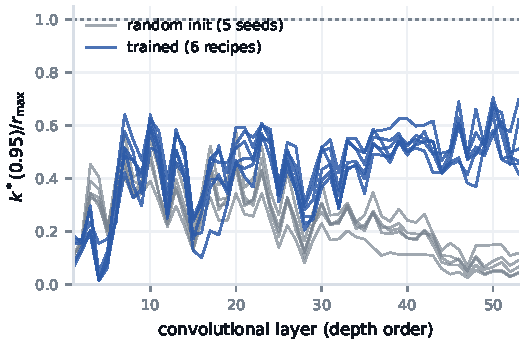
\includegraphics[width=0.92\columnwidth]{fig1_profile.pdf}
  \caption{$k^*(0.95)/r_{\max}$ against layer index for the six ResNet-50
  recipes (thin lines) and their five random initialisations (grey), on the
  same $6{,}400$ images. The dashed rule at $1.0$ marks full use of the
  attainable rank.}
  \label{fig:profile}
\end{figure}

\emph{Exploratory; full set and subset.} Fig.~\ref{fig:profile} shows the
profile in units of attainable rank for the one case with an error bar,
six ResNet-50 recipes on the same images. Across recipes the per-layer
standard deviation of $k^*(0.95)/r_{\max}$ has median $0.053$ (maximum
$0.123$); the adjacent-layer step within one recipe has median $0.087$.
The spread between independently trained networks is thus $0.6$ of the
step between neighbouring layers, which settles what a single checkpoint
can support: the value at one layer against the next is not reproducible
and is not reported below; the ordering over the profile is (pairwise
$\rho = 0.79$--$0.92$), and so is the level, which moves with the recipe
from $0.38$ (\texttt{torchvision} V1) to $0.48$ (A1). Across
the eleven families (columns $T$ and $R$ of Table~\ref{tab:families}) the
median $k^*(0.95)/r_{\max}$ of a trained network's dense convolutions lies
between $0.33$ (Wide-ResNet-50-2) and $0.72$ (MobileNetV2), and the
depthwise convolutions of the inverted-residual families below their dense
ones, at $0.20$--$0.42$.

\subsection{Pooled Versus Position-Sampled Covariance}
\label{sec:estimator}

\emph{Pre-registered; full validation set.} The registered hypothesis was
that the estimator changes the \emph{shape} of the profile and so accounts
for the published disagreement. Both estimators were computed on the same
forward pass and layers.

\emph{Level.} Over the 19 trained checkpoints the pooled $k^*(0.95)/C$ is
strictly lower on $687$ of $703$ dense and $79$ of $80$ depthwise
convolutions passing the pooled gate. Of the 16 dense exceptions 14 are
ties (ten in DenseNet-121 at $C = 32$, where one channel is $0.031$ of the
range, four at the first bottleneck of ResNet-50 recipes) and two are
reversals, of one channel in DenseNet-121 and of 23 at the reducing
$1\!\times\!1$ of the last block (\texttt{layer4.2.conv1}) of the
\texttt{torchvision} V2 ResNet-50. Table~\ref{tab:pooling} puts the drop
beside each profile's own step under both denominators. Under $C$ the
inverted-residual networks appear to show almost nothing (drop
$0.06$--$0.09$ against a step of $0.5$--$0.7$), but that step is the $1/6$
expansion sawtooth of Section~\ref{sec:rmax}; under $r_{\max}$ the same
networks drop by $1.25$--$2.1$ times their step, in line with the others
(median $2.2$). DenseNet-121 alone stays below one, its step being the
structural alternation of $128$- and $32$-channel layers.
\begin{table*}[t]
  \centering
  \caption{Pooling lowers the level. Per trained checkpoint: dense
  convolutions passing the pooled gate on which the pooled $k^*(0.95)$ is
  strictly lower; the median drop and the profile's own adjacent-layer step,
  under $C$ and under $r_{\max}$; and their ratio.}
  \label{tab:pooling}
  \footnotesize
  % Generated by scripts/checkpoint_analysis.py --latex-pooling.  Do not edit by hand.
\begin{tabular}{llrrrrrrr}
\toprule
Model & Recipe & lower & drop$/C$ & step$/C$ & ratio & drop$/r_{\max}$ & step$/r_{\max}$ & ratio \\
\midrule
VGG-16 (BN) & tv & 13/13 & 0.281 & 0.074 & 3.79 & 0.281 & 0.054 & 5.24 \\
ResNet-18 & tv & 20/20 & 0.285 & 0.172 & 1.66 & 0.289 & 0.141 & 2.06 \\
VGG-16 & tv & 13/13 & 0.254 & 0.068 & 3.71 & 0.254 & 0.051 & 4.98 \\
ResNet-34 & A1 & 36/36 & 0.361 & 0.109 & 3.30 & 0.361 & 0.102 & 3.56 \\
ResNet-50 & tv V1 & 42/42 & 0.131 & 0.137 & 0.96 & 0.163 & 0.078 & 2.09 \\
ResNet-50 & tv V2 & 40/42 & 0.192 & 0.148 & 1.30 & 0.223 & 0.090 & 2.48 \\
ResNet-50 & A1 & 41/42 & 0.193 & 0.150 & 1.29 & 0.217 & 0.102 & 2.13 \\
ResNet-50 & A3 & 41/42 & 0.182 & 0.145 & 1.26 & 0.203 & 0.094 & 2.17 \\
ResNet-50 & GluonCV & 41/42 & 0.169 & 0.141 & 1.20 & 0.209 & 0.094 & 2.23 \\
ResNet-50 & SSL ft & 42/42 & 0.191 & 0.182 & 1.05 & 0.234 & 0.094 & 2.50 \\
ResNet-101 & tv & 76/76 & 0.136 & 0.078 & 1.74 & 0.158 & 0.066 & 2.38 \\
Wide-ResNet-50-2 & tv & 36/36 & 0.095 & 0.104 & 0.92 & 0.119 & 0.102 & 1.17 \\
ResNeXt-50 32x4d & tv & 36/36 & 0.146 & 0.193 & 0.75 & 0.184 & 0.158 & 1.16 \\
DenseNet-121 & tv & 109/120 & 0.148 & 0.297 & 0.50 & 0.148 & 0.297 & 0.50 \\
MobileNetV2 & RA & 34/34 & 0.055 & 0.682 & 0.08 & 0.231 & 0.109 & 2.11 \\
MobileNetV3-L & RA & 31/31 & 0.089 & 0.514 & 0.17 & 0.188 & 0.150 & 1.25 \\
EfficientNet-B0 & RA & 28/28 & 0.059 & 0.625 & 0.09 & 0.187 & 0.125 & 1.50 \\
ConvNeXt-T & in1k & 4/4 & 0.152 & 0.061 & 2.49 & 0.204 & 0.026 & 7.85 \\
ConvNeXt-T & in22k ft & 4/4 & 0.152 & 0.102 & 1.50 & 0.204 & 0.102 & 2.01 \\
\bottomrule
\end{tabular}

\end{table*}

\emph{Shape.} The registered test, a rank correlation between depth and
the pooled-minus-sampled difference over all gated layers, is not
significant in any of the three first-round architectures with enough
dense layers ($|\rho| \le 0.35$, $p \ge 0.24$), and for VGG-16 the sign
is opposite to the one a ``pooling removes the terminal collapse''
account needs. The registered hypothesis is not supported. What holds is narrower
and more useful: pooling averages away the within-image spatial variance
and lowers the profile at every layer by more than the profile's own step,
so the two published literatures' numbers are not on one scale whatever
their shapes. Two limits: the pooled gate excludes the $1024$- and
$2048$-channel layers (eleven of ResNet-50's 53), where the difference
would be largest; and adjacent layers are correlated, so the per-checkpoint
Wilcoxon $p$-values (at most $1.2 \times 10^{-4}$) are optimistic and the
counts carry the claim.

\subsection{Convolution Output Versus Block Output}
\label{sec:blockout}

\emph{Exploratory; full validation set.} The bound binds the expansion
convolution's output and not the block output, which adds the shortcut and
rectifies. Both were recorded for all $161$ bottleneck blocks of the nine
bottleneck networks. That the sum of a shortcut and a rectified expansion
has higher rank than the expansion is certain; the size of the gap, and
that the two literatures reading the two tensors had not noticed they
read different objects, are the findings. In every block the block output exceeds the rank bound
of its own last convolution: at $\tau = 0.999$ the expansion output has
median $k^*/C$ of $0.23$ (ceiling $0.25$) in the ResNet-50 and ResNet-101
checkpoints and the block output $0.96$--$0.99$, a factor of $4.1$, the
expansion ratio; in Wide-ResNet-50-2 and ResNeXt-50 (ceiling $0.5$) the
factor is $2.3$--$2.4$; under $k^*(0.95)/C$ the values rise from
$0.09$--$0.19$ to $0.58$--$0.72$, higher in $161$ of $161$. Along the depth
of ResNet-50 the expansion outputs sit at their ceiling from the second
block on while the block outputs rise from $0.72$--$0.92$ to $0.99$
(supplement, Fig.~S2), so the block-level profile of a bottleneck network
is a shallow rise toward full rank, the shape \cite{elmoznino2024highDim}
report at this tensor. Neither tensor is wrong, but the two profiles differ
by the expansion ratio at 20 of ResNet-50's 53 layers, and a profile that
does not state its tensor is not comparable with one read at the other.

\subsection{Agreement Between Summary Statistics}
\label{sec:metrics}

\emph{Pre-registered; full validation set.} The plan asked whether
$k^*(0.95)$ and the participation ratio order the layers of a network the
same way and predicted they need not, PR being set by the head of the
spectrum and $k^*$ counting to its tail. The registered summary, recipe
agreement across the six ResNet-50 checkpoints, is $\rho = 0.85$ for
$k^*(0.95)/r_{\max}$, $0.86$ for $\mathrm{PR}/C$ and $0.89$ for
$\mathrm{erank}/C$: each statistic gives a reproducible profile.

\emph{Exploratory (plan Section~11).} Reproducible is not interchangeable.
On the $894$ gate-passing dense convolutions of 21 checkpoints we computed
PR, its finite-sample correction \cite{chun2026estimating}, effective
rank, RankMe \cite{garrido2023rankme} and the $\alpha$-ReQ exponent
\cite{agrawal2022alphaReq} from the same spectra (supplement, Table~S3).
Within a network PR and the ruler do not order layers alike (per-network
$\rho$ median $0.41$; $-0.52$ on the ImageNet VGG-16, where PR falls with
depth while $k^*(0.999)$ rises); effective rank sits between ($0.63$);
RankMe orders layers as the ruler does ($0.94$); $\alpha$ is the most
stable quantity across recipes ($0.97$) but is a slope, not a count. The
finite-sample correction changes PR by at most $0.03\%$ at the gate, and
the pooling count of Section~\ref{sec:estimator} is the same under every
statistic ($687$, $669$, $688$ of $703$). We conclude that the registered
hypothesis holds in its mechanism and fails in its predicted direction:
head-weighted statistics do reorder layers, but on a plain network the PR
profile falls with depth rather than rising, so the statistic explains
part of the published disagreement and not its sign. Every conclusion
below for $k^*(\tau)/r_{\max}$ transfers to RankMe and to the pooling
count, and not to PR or $\alpha$.

\subsection{Depthwise and Dense Convolutions}
\label{sec:dwsplit}

\emph{Exploratory; full set and subset.} A depthwise layer does not mix
channels, and three architectures show why the two kinds cannot share an
axis. Eighteen of ConvNeXt-T's 22 convolutions are depthwise, four dense,
and the groups do not overlap (median $k^*(0.95)/C$ $0.71$ against
$0.31$); in MobileNetV3-Large and EfficientNet-B0 the sign reverses, the
depthwise layers at $0.19$ and $0.16$ of $r_{\max}$ against $0.51$ and
$0.56$ for the $1\!\times\!1$ layers. Interleaved, either pair produces a
sawtooth that is not a property of the representation. Kept apart, the
split also weakens ConvNeXt-T's trained-versus-untrained comparison: its
four dense convolutions are all higher than at initialisation in both
checkpoints ($p = 0.06$ with four layers), its depthwise ones higher in
$13$ ($p = 0.013$) and $12$ ($p = 0.21$) of 18.

\subsection{Trained Versus Initialised Profiles}
\label{sec:learned}

\emph{Exploratory; full validation set for the paired test, the
$6{,}400$-image subset with seeds for the rest.}\label{sec:trained}

\emph{Level.} Against one random initialisation on the full validation set,
each of the six trained ResNet-50 recipes is higher on $45$ to $50$ of its
53 dense convolutions (Wilcoxon $p \le 4 \times 10^{-8}$). The median
difference in $k^*(0.95)/C$, $+0.10$ to $+0.20$, is smaller than those
profiles' adjacent-layer step of $0.20$--$0.27$; in units of attainable
rank, on the subset with five random seeds, the level is $0.23$ at
initialisation and $0.47$ trained against a step of $0.09$. The paired
test over all layers carries the claim.

\emph{Ordering.} Higher says nothing about shape. For each family three
rank correlations between $k^*(0.95)/r_{\max}$ profiles were computed over
its dense convolutions on the same images: random against random (R--R),
the ceiling a comparison with one draw can reach; trained against trained
(T--T), whether the recipes share a profile; and trained against random
(T--R), the question (Table~\ref{tab:families}). A family with T--R near
R--R has an ordering set by the architecture; one with T--R far below both
has learned it. Three behaviours appear.

\begin{table*}[t]
  \centering
  \caption{Is the ordering of layers learned? Median Spearman $\rho$ between
  $k^*(0.95)/r_{\max}$ profiles over a family's $L$ dense convolutions, on the
  same $6{,}400$ images: random-vs-random over $n_R$ seeds, trained-vs-trained
  over $n_T$ checkpoints, and trained-vs-random over all pairs. $T$ and $R$
  are the median levels. Depthwise rows are reported separately. VGG-16's
  two checkpoints are with and without BN. ConvNeXt-T, with four dense
  convolutions, is omitted: a rank correlation over four layers is
  uninformative (Section~\ref{sec:dwsplit}).}
  \label{tab:families}
  \footnotesize
  % Generated by scripts/checkpoint_analysis.py.  Do not edit by hand.
\begin{tabular}{llrrrrrrrrrr}
\toprule
 & & & & & \multicolumn{3}{c}{$k^*/r_{\max}$} & \multicolumn{2}{c}{$k^*/C$} & & \\
\cmidrule(lr){6-8}\cmidrule(lr){9-10}
Family & Block & $L$ & $n_T$ & $n_R$ & R--R & T--T & T--R & T--R & T--R$_{\rm stage}$ & $T$ & $R$ \\
\midrule
ResNet-50 & bottleneck & 53 & 6 & 5 & +0.94 & +0.84 & -0.08 & +0.57 & +0.27 & 0.47 & 0.23 \\
ResNet-18 & basic & 20 & 6 & 3 & +0.98 & +0.91 & +0.73 & +0.81 & +0.75 & 0.54 & 0.33 \\
ResNet-34 & basic & 36 & 5 & 3 & +0.96 & +0.92 & +0.61 & +0.67 & +0.55 & 0.58 & 0.41 \\
VGG-16 ($\pm$BN) & plain & 13 & 2 & 3 & +0.79 & +0.96 & +0.75 & +0.76 & --- & 0.39 & 0.29 \\
DenseNet-121 & dense & 120 & 2 & 3 & +0.94 & +0.91 & +0.71 & +0.71 & --- & 0.66 & 0.41 \\
MobileNetV3-L & inverted residual & 31 & 3 & 3 & +0.75 & -0.19 & -0.26 & +0.55 & --- & 0.50 & 0.53 \\
\quad depthwise &  & 15 & 3 & 3 & +0.37 & +0.50 & -0.05 & -0.05 & --- & 0.19 & 0.41 \\
EfficientNet-B0 & inverted residual & 33 & 2 & 3 & +0.97 & +0.10 & +0.14 & +0.69 & --- & 0.54 & 0.55 \\
\quad depthwise &  & 16 & 2 & 3 & +0.97 & -0.10 & -0.12 & -0.12 & --- & 0.16 & 0.35 \\
\bottomrule
\end{tabular}

\end{table*}

(i)~\emph{Plain, basic-residual and dense families learn a level, not an
ordering.} VGG-16, ResNet-18, ResNet-34 and DenseNet-121 have T--R of
$0.61$--$0.75$ against ceilings of $0.79$--$0.98$, and training raises the
median level by $0.09$ to $0.19$, more than the profile's own step in all
but DenseNet-121. This is the observation Ansuini \emph{et al.}
\cite{ansuini2019intrinsic} made on VGG-16's PC-ID profile, now with seeds.

(ii)~\emph{The ImageNet ResNet-50 checkpoints learn their ordering.} T--T
is $0.84$, T--R $-0.08$ (range $-0.31$ to $+0.33$ over 30 pairs), R--R
$0.94$; every random draw falls with depth ($\rho_{\rm depth}$ $-0.53$ to
$-0.81$) and every trained recipe rises ($+0.56$). Ranking within stages,
where no bound confound is possible, leaves $0.27$ against a ceiling of
$0.75$, so the reordering is real within stages as well. Depth is not the
cause, since ResNet-101 agrees with its initialisation \emph{more}
($0.20$) and Wide-ResNet-50-2 and ResNeXt-50 more still ($0.33$, $0.46$),
the four bottleneck families ordering as a gradient below every other
family; nor is the kernel role, since in ResNet-50 both $3\!\times\!3$ and
$1\!\times\!1$ layers reorder while in DenseNet-121 only the
$3\!\times\!3$ layers do.

(iii)~\emph{Inverted-residual checkpoints agree weakly or not at all.}
MobileNetV3-Large's four checkpoints share no profile (T--T $-0.18$, R--R
$0.75$) and EfficientNet-B0's five agree moderately ($0.40$, R--R $0.97$);
the $1\!\times\!1$ levels span $0.18$--$0.65$ and $0.10$--$0.73$ under one
architecture and dataset, and training halves the depthwise layers. These
checkpoints differ in pre-training data, length and framework, so this is
a statement about the checkpoints one can download.

\emph{Is the block the cause?} The plan (its Section~9.1) registered, before
its data, the experiment that separates the block from everything else
that varies between public checkpoints: a basic-block ResNet $[6,6,6,6]$
and a bottleneck ResNet-50 $[3,4,6,3]$ with the same stage widths, stem
and convolution count ($52$ and $53$), and a CIFAR MobileNetV2, three
seeds each under the recipe of Section~\ref{sec:repro-garg} (supplement,
Table~S9). H9.1, that the bottleneck network's T--R lies below the basic
network's, fails: $0.55$ ($0.46$--$0.57$) against $0.50$ ($0.38$--$0.54$),
$p = 0.2$, MobileNetV2 $0.44$; the CIFAR bottleneck's level \emph{falls}
on training ($0.20 \to 0.16$) and its depth trend flattens rather than
reversing. H9.2 holds: the three MobileNetV2 seeds share their profile at
$\rho = 0.99$--$1.00$ against a ceiling of $0.68$, so an inverted-residual
network under one recipe has a profile and the public disagreement is the
recipes'. We conclude that the bottleneck block is not sufficient: under
one CIFAR-10 recipe it keeps its initial ordering as the basic block does.
What reorders the ImageNet ResNet-50 checkpoints is therefore not the
block alone but the dataset or the ImageNet recipes, alone or in
interaction with the block, which this experiment does not separate
(Section~\ref{sec:limits}). One block-specific behaviour is on record:
the CIFAR bottleneck's level falls on training where the basic block's
rises ($0.21 \to 0.32$).

\emph{When.} A VGG-16 (BN) on CIFAR-10 has its final ordering by epoch 40
($\rho$ to the final profile $0.98$ from then on) while accuracy still
rises from $84\%$ to $94\%$, and its final profile agrees with the initial
one at $0.93$. The nine controlled runs agree with seeds (supplement,
Fig.~S5): after one epoch every profile is \emph{anti}-correlated with
its initial one ($-0.50$), with a rising depth trend and a doubled level;
by epoch 15--20 the trend falls again and the agreement with
initialisation climbs to $0.6$--$0.9$, drifting to its final
$0.50$--$0.54$; the profile settles at epoch 40--60 while accuracy is
$84$--$88\%$. The rising trend of the trained ImageNet ResNet-50 is thus
present transiently in every CIFAR-10 network and undone. The last three
layers end at $k^*(0.95)/C$ of $0.05$--$0.07$: the terminal collapse of
\cite{garg2019lowEffort} is present in our CIFAR-10 VGG-16 and absent in
our ImageNet VGG-16 ($0.44$--$0.53$); Section~\ref{sec:a18} ties it to
few classes and long optimisation. One caution: at $\tau = 0.999$
ResNet-50's T--R is $0.25$ rather than $-0.07$, the ceiling compressing
both profiles.

\subsection{Functional Calibration by Truncation}
\label{sec:projection}

\emph{Exploratory; the $6{,}400$-image subset.} Whether the directions the
statistic discards carry function can be checked at inference by
replacing each convolution output $y$ with
$\bar y + U_k U_k^{\top}(y - \bar y)$, $U_k$ its top-$k$ principal channel
directions, the response-PCA truncation of Zhang \emph{et al.}
\cite{zhang2016accelerating}, here with $k = k^*(\tau)$ from the
measurement, at every dense convolution at once, without fine-tuning. The
scale of the answer is fixed to first order by the discarded variance.

\begin{proposition}[first-order effect of truncation]
\label{prop:truncation}
Let $z$ be the output of layer $\ell$ at a position, $\Sigma_\ell = \sum_i \lambda_i u_i u_i^{\top}$ its covariance, $r = (I - U_k U_k^{\top})(z - \bar z)$ the discarded component, and $J_\ell$ the Jacobian of the logits with respect to $z$. Then $\mathbb{E}\|r\|^2 = (1 - \tau_k)\operatorname{tr}\Sigma_\ell$ with $\tau_k$ the captured fraction, and to first order
\[
  \mathbb{E}\|J_\ell r\|^2 = \operatorname{tr}\bigl(J_\ell \Sigma_\ell^{\perp}(k) J_\ell^{\top}\bigr) \le \|J_\ell\|_{\rm op}^2 (1 - \tau_k) \operatorname{tr}\Sigma_\ell,
\]
where $\Sigma_\ell^{\perp}(k) = \sum_{i > k} \lambda_i u_i u_i^{\top}$; truncating $L$ layers at once perturbs the logits by at most $\sum_\ell (\mathbb{E}\|J_\ell r_\ell\|^2)^{1/2}$ in root mean square.
\end{proposition}

Between $\tau = 0.999$ and $0.95$ the discarded energy per layer differs by
a factor of $50$ and the layers add, so the two thresholds are an order of
magnitude apart in what they inject; on the A1 recipe the linearisation
agrees with the actual logit change in rank order across layers at
$\rho = 0.99$--$1.00$ at every $\tau$. Covariances were accumulated on one
half of the subset and the truncated network evaluated on the other, with
a control that truncates to $k^*(\tau)$ random directions
(supplement, Table~S11; exact McNemar test per cell).


At $\tau = 0.999$ the truncation keeps $84$--$93\%$ of each layer's
attainable rank and accuracy is unchanged in six of eight checkpoints
(ResNet-18, VGG-16 and four of the six ResNet-50 recipes: $-0.3$ to
$+0.2$ points on $3{,}200$ images, exact McNemar $p \ge 0.15$); the two
ResNet-50 checkpoints
trained with the A1 and A3 recipes of Wightman \emph{et al.}
\cite{wightman2021rsb} lose $1.7$ points each ($p < 10^{-4}$), so binary
cross-entropy with heavy augmentation places function in directions
holding under $0.1\%$ of the variance. Random directions of the same
dimension give chance throughout: what is retained is the subspace, not
the count. Below $0.999$ the cost is recipe-dependent, from $1.6$--$5.2$
points to a fall to $11\%$ at $0.99$, and at the registered $0.95$ three
checkpoints lose $19$--$21$ points and five collapse. We conclude that
$k^*(0.999)$ bounds the width a conventionally trained network uses and
undercounts it by about two points for the RSB recipes, while
$k^*(0.95)$ orders layers and tracks training but says nothing about
removable width. This is not a compression or pruning result; whether a
narrower network trained from scratch reaches the same accuracy is the
question of Section~\ref{sec:a18}.

\subsection{Decomposition of the Effective Width}
\label{sec:decompose}

\emph{Exploratory; the $6{,}400$-image subset.} At the tensor this paper
reads, the channel covariance is an exact function of the kernel and of
the receptive-field patch. With $W \in \mathbb{R}^{C_{\rm out} \times d}$
the kernel as a matrix, $d = C_{\rm in} k_h k_w$, and $\Sigma_{\rm patch}$
the $d \times d$ covariance of the patch vector at a sampled position,
\begin{equation}
  \Sigma_{\rm out} = W\, \Sigma_{\rm patch}\, W^{\top}.
  \label{eq:decomp}
\end{equation}
The bound of Section~\ref{sec:rmax} is the rank of the right-hand side.
Write $W = P W_{\circ}$ for the polar decomposition, $P = (WW^{\top})^{1/2}$
and $W_{\circ}$ the nearest semi-orthogonal matrix to $W$, with
$r = \operatorname{rank} W$ and $\sigma_{\max} \ge \sigma_{\min} > 0$ its
extreme nonzero singular values.

\begin{proposition}[the kernel reweights the counterfactual spectrum]
\label{prop:ostrowski}
Let $\Sigma_{\circ} = W_{\circ} \Sigma_{\rm patch} W_{\circ}^{\top}$. Then
$\Sigma_{\rm out} = P \Sigma_{\circ} P$, and for $i \le r$ there are
$\theta_i \in [\sigma_{\min}^2, \sigma_{\max}^2]$ with
$\lambda_i(\Sigma_{\rm out}) = \theta_i\, \lambda_i(\Sigma_{\circ})$; both
spectra vanish beyond $r$.
\end{proposition}

\begin{corollary}
\label{cor:kstar}
With $\kappa = \sigma_{\max}/\sigma_{\min}$, $\tau' = \kappa^2\tau / (1 - \tau + \kappa^2 \tau)$ and $\tau'' = \tau / (\kappa^2 (1 - \tau) + \tau)$,
$k^*(\tau''; \Sigma_{\circ}) \le k^*(\tau; \Sigma_{\rm out}) \le k^*(\tau'; \Sigma_{\circ})$ for every $\tau \in (0, 1)$.
If $\kappa = 1$ then $k^*(\tau; \Sigma_{\rm out}) = k^*(\tau; \Sigma_{\circ})$, and if moreover
$C_{\rm out} \ge d$ then $k^*(\tau; \Sigma_{\rm out}) = \min(k^*(\tau; \Sigma_{\rm patch}), r_{\max})$.
\end{corollary}

Two further statements in the supplement complete the picture:
$\Sigma_{\circ}$ depends on the kernel only through which input
directions it keeps (Proposition~S1), and the rank of layer $\ell + 1$'s
output is at most $k_h k_w$ times the rank of layer $\ell$'s activation
covariance (Proposition~S2), the bound that binds at initialisation.
Proposition~\ref{prop:ostrowski} says the kernel acts on
the width only through the spread of its singular values, and
Corollary~\ref{cor:kstar} is the exact form of the claim that an isometric
kernel passes the effective width of its input through unchanged, the aim
of orthogonality regularisation (Section~\ref{sec:where}), which reaches
the ceiling only if the input is also white. On the 465 dense convolutions of the ten checkpoints in
Table~S12 the eigenvalue ratios of
Proposition~\ref{prop:ostrowski} lie within
$[\sigma_{\min}^2, \sigma_{\max}^2]$ on 464 and the corollary holds on 465
at both thresholds, informatively on 246 at $\tau = 0.95$ (median
$\kappa = 10.6$); twenty-four trained layers have numerically null kernel
directions and no random layer does, so training empties some kernel
directions outright, the low-rank bias of Huh \emph{et al.}
\cite{huh2023lowRank} seen in the kernel.

For every dense convolution we accumulated $\Sigma_{\rm patch}$
($n/d \ge 67$) and compared four quantities: the measured $k^*/r_{\max}$,
recomputed from Equation~\eqref{eq:decomp}; the same for $WW^{\top}$, the
width under white patches; for $\Sigma_{\rm patch}$ capped at $r_{\max}$;
and for $W_{\circ}\Sigma_{\rm patch}W_{\circ}^{\top}$, the width the layer
would have with its kernel orthogonalised and its input left as it is
(Table~S12; supplement, Fig.~S6).

Three things follow. The identity checks the pipeline:
$k^*(0.95)/r_{\max}$ recomputed from $W$ and an independently accumulated
$\Sigma_{\rm patch}$ reproduces the measured value within $0.008$ on every
layer. Training moves the bottleneck from the data to the kernel: at
initialisation the patch covariance is far from full-rank (median $0.28$
of $r_{\max}$ for ResNet-50), the random kernel nearly isotropic ($0.86$),
and the measured width follows the data ($\rho = 0.94$) rather than the
kernel ($0.44$), the untrained patch covariance losing rank with depth,
which is why every random profile in Section~\ref{sec:learned} falls with
depth; in every trained checkpoint the patch covariance is full-rank at
the $95\%$ criterion (median $1.00$) and the measured width follows the
kernel spectrum ($\rho = 0.81$--$0.97$ in six of nine checkpoints), so the
ordering of a trained profile is, to first approximation, the ordering of
the kernels' Gram spectra. And the level is set jointly: a trained kernel
under white patches would give $0.69$--$0.86$, the measured value is
$0.42$--$0.70$, and orthogonalising the kernel with the measured patches
gives $0.75$--$0.87$, above the measured value in $401$ of $412$ dense
convolutions; the trained kernel's high-gain directions are aligned with
the high-variance directions of its input, so the two factors compound.

\emph{Alignment, measured (plan Section~9.6; the registered sign was
wrong).} With $W = \sum_i s_i u_i v_i^{\top}$, let $\rho_{\rm align}$ be
the Spearman correlation over the retained right singular directions
between the kernel's gain $s_i^2$ and the input variance the direction
carries, $v_i^{\top}\Sigma_{\rm patch}v_i$. The plan registered
$\rho_{\rm align} < 0$; the reasoning had the sign backwards, since it is
amplification of the principal directions that steepens the output
spectrum below the isometric counterfactual, and as registered the
prediction fails in $0$ of $48$ networks. Reported post hoc, the opposite
holds strongly: over the 19 ImageNet checkpoints the network-median
$\rho_{\rm align}$ is $+0.91$, significant at $p < 0.01$ in $43$ of the
$48$ trained networks measured, while every one of 20 random draws has
$|\rho_{\rm align}| < 0.1$; the exceptions are the inverted-residual
families ($+0.11$ to $+0.61$), whose public checkpoints share no profile.
Along training the alignment reaches $90\%$ of its final value by epoch
$7$--$15$, before the profile settles and long before the representation
does (CKA to the final network reaches $0.9$ only in annealing; P9.23
fails in all nine runs). This is the behaviour Saxe \emph{et al.}
\cite{saxe2014exact} derive for gradient descent on a linear layer, here
measured in trained convolutions with its size and its time course. We conclude
that the trained kernel's gain is aligned with its input's principal
directions, and that the measured width sits below the isometric
counterfactual because the kernel sharpens the input spectrum rather than
flattening it.

\emph{The prediction, tested (plan Section~9.2).} An orthogonal kernel
decorrelates its output when the input is white \cite{huang2018own};
Table~S12 shows the trained input is full-rank but not
white, so orthogonalisation should add about $0.3\,r_{\max}$, not reach
the ceiling. VGG-16 (BN) and the basic ResNet of Table~S9 were trained on
CIFAR-10 without penalty, with soft orthogonality SO
($\|WW^{\top} - I\|_F^2$, $\lambda = 10^{-4}$) and with SRIP
($\lambda = 10^{-2}$) \cite{bansal2018orthogonality}, three seeds each,
and the penalised $k^*(0.95)/r_{\max}$ compared with the \emph{ortho}
counterfactual of the unpenalised network of the same seed
(supplement, Table~S10). P9.3, that SO lands within $0.1$ of the
counterfactual, fails: both penalties raise the level from $0.35$--$0.36$
to $0.53$--$0.56$ (SO) and $0.42$--$0.54$ (SRIP), half of the predicted
gain, because at these strengths the kernels' effective rank rises only
to $0.80$--$0.85$ of $r_{\max}$ and the alignment is untouched
($|\rho_{\rm align}|$ differs by $+0.002$ over the 195 SO layers). What
the counterfactual does predict is the \emph{ordering} of the gains:
across the SO layers the gain obtained correlates with the gain predicted
at $\rho = 0.72$ (ResNet) and $0.91$ (VGG-16), across the SRIP layers it
does not ($-0.14$, $-0.19$), the form in which P9.4 holds; P9.5 holds,
accuracy moving by $-0.1$ to $+0.3$ points uncorrelated with the width
gained. The counterfactual is an upper bound that a soft penalty
approaches by half, in the layers it names; an exact isometry constraint
\cite{huang2020oni} was not run.


\subsection{The Profile as a Diagnostic}
\label{sec:diagnostic}

\emph{Exploratory.} Pooling the six ResNet-50 recipes by role and stage
(supplement, Table~S5), $k^*(0.999)/r_{\max}$ reads above $0.9$ on 29 of
the 53 layers in every recipe and $0.95$--$0.97$ at every $3\!\times\!3$
convolution. The width not used sits at the entry of the network and in
its projection shortcuts: the stem at $0.49$, the first block of stage~1
at $0.40$--$0.61$, and the four stride-2 shortcuts at $0.61$ to $0.94$
from stage 1 to 4, the only layers below $0.7$ in all six recipes. The reading
is not ``ResNet-50 is half idle'' but ``its entry and its shortcuts are
wider than what passes through them, by about two, in every recipe''.
Beside network slimming \cite{liu2017slimming} on the same CIFAR-10
VGG-16, the ruler agrees where the profile is decided (both cut the first
convolution to a fifth or a third of 64 and collapse the last resolution
to $32$--$40$ of $512$) and disagrees at the fourth resolution, since the
ruler reports the rank the activations span and slimming what can be
removed when the network is retrained around the removal; the rank of a
feature map is also HRank's pruning score \cite{lin2020hrank}, read per
filter where the ruler reads per layer. Whether the
ruler's widths retrain to full accuracy is the next section.

\subsection{Retraining at the Measured Widths}
\label{sec:a18}

\emph{Pre-registered (plan Sections~9.5, 9.7, 9.8, 9.9, 9.11--9.13); three
seeds per arm unless stated.} The widths above were read off one trained
network. The plan asked whether a network built at them and trained from
scratch keeps the accuracy of the full one, and whether the per-layer
allocation matters. VGG-16 (BN) on CIFAR-10 under the recipe of
Section~\ref{sec:repro-garg}, four arms: full width; the ruler's
$\lceil k^*(0.999)_\ell \rceil$ read on the seed-0 full network over
$6{,}400$ training images ($34.5\%$ of the parameters); a uniform cut to
the same parameter count; and the ruler at $\tau = 0.95$ ($0.63$M
parameters). Table~\ref{tab:a18} gives the outcome.

\begin{table}[t]
  \caption{Widths from the ruler, retrained from scratch (pre-registered, plan Sections~9.5, 9.7 and 9.8): VGG-16 (BN), three seeds per arm, test accuracy at epoch 100 as mean $\pm$ SD over seeds, and the median over layers of the retrained network's own $k^*(0.999)/r_{\max}$. MACs are multiply-adds per $32 \times 32$ image; img/s is inference throughput measured on one RTX 4090 at batch 256. The CIFAR-10 full-width arm is the untreated arm of the penalty test (supplement, Table~S10). The lower block (plan Section~9.11) is ResNet-18 on ImageNet-1k under the \texttt{torchvision} reference recipe, two seeds per arm, final-epoch top-1 as mean $\pm$ SD of the two seeds (the two full-width seeds differ by $0.60$ points); its MACs are per $224 \times 224$ image, and its throughput and retrained level were not measured.}
  \label{tab:a18}
  \centering
  \scriptsize
  \setlength{\tabcolsep}{2.5pt}
  % Generated by scripts/checkpoint_analysis.py --latex-a18.  Do not edit by hand.
\begin{tabular}{lrrrrr}
\toprule
Arm & params & MACs & img/s & accuracy (\%) & $k^*(0.999)/r_{\max}$ \\
\midrule
\multicolumn{6}{@{}l}{\emph{CIFAR-10 (plan 9.5, 9.8)}} \\
full width & 14.73M & 313M & 61k & 93.77 $\pm$ 0.05 & 0.74 \\
ruler, $\tau = 0.999$ & 5.09M & 189M & 82k & 93.55 $\pm$ 0.16 & 0.85 \\
uniform cut & 5.00M & 107M & 86k & 93.20 $\pm$ 0.25 & 0.92 \\
ruler, $\tau = 0.95$ & 0.63M & 31M & 237k & 91.62 $\pm$ 0.29 & 0.98 \\
ruler after ReLU, $\tau = 0.999$ & 9.92M & 276M & 65k & 93.84 $\pm$ 0.04 & 0.75 \\
\midrule
\multicolumn{6}{@{}l}{\emph{CIFAR-100 (plan 9.7, 9.8)}} \\
full width & 14.77M & 313M & 62k & 73.23 $\pm$ 0.10 & 0.92 \\
ruler, $\tau = 0.999$ & 12.88M & 232M & 67k & 72.64 $\pm$ 0.20 & 0.93 \\
uniform cut & 12.99M & 275M & 65k & 73.24 $\pm$ 0.32 & 0.93 \\
ruler, $\tau = 0.95$ & 1.86M & 33M & 208k & 67.42 $\pm$ 0.40 & 0.97 \\
ruler after ReLU, $\tau = 0.999$ & 14.62M & 301M & 57k & 73.49 $\pm$ 0.29 & 0.92 \\
\bottomrule
\end{tabular}

\end{table}

\emph{CIFAR-10.} P9.6, that the ruler's widths lose under $0.3$ points
with no seed more than $0.5$ below, holds ($93.55$ against $93.77$); P9.8,
that the $\tau = 0.95$ widths lose at least one point, holds with $2.15$,
the training-side counterpart of Section~\ref{sec:projection}; P9.7, that
every uniform-cut seed falls below every ruler seed, fails by one image
(eight pairs of nine, the ninth an exact tie), so by the registered rule
we do not claim the allocation is needed at this budget, which is what
Liu \emph{et al.} \cite{liu2019rethinkingPruning} report for pruned
architectures retrained from scratch. The retrained
network does not fill the ruler's widths ($0.85$ of $r_{\max}$ against
$0.74$ at full width): the count is re-made by training rather than
inherited.

\emph{CIFAR-100 (plan Section~9.7).} With widths re-read from a CIFAR-100
network the last five layers are nearly full ($466$--$490$ of $512$,
against $40$ on CIFAR-10), the ruler removes $13\%$ of the parameters, and
the answer reverses: P9.14 fails (the ruler arm loses $0.59$ points),
P9.15 fails in the direction opposite to P9.7 (the uniform cut is above
the ruler in nine pairs of nine), and P9.16 holds with $5.8$ points.

\emph{The tensor the next layer consumes (plan Section~9.8).} The measurement
exposes the cause: the ruler reads the convolution output, where the bound
holds, but the next layer consumes the post-activation tensor, and the
ReLU raises the rank where the input is a low-rank RGB patch (the first
convolution spans $14$--$15$ directions at $\tau = 0.999$, its ReLU output
$47$--$48$). A layer narrowed to the rank of its own output caps what the
next layer receives. The registered fifth arm reads the widths after the
ReLU ($67\%$ of the parameters); P9.17, within $0.3$ of full width, and
P9.18, above the convolution-output widths seed for seed, both hold
($93.84$ against $93.77$), and on CIFAR-100 the post-activation widths are
$99\%$ of the full ones, so that arm is not evidence. We conclude that a
width read at $\tau = 0.999$ is the rank the activations span: at the
convolution output it is the width the layer \emph{produces}, and a
network built at it loses where the nonlinearity had raised the rank;
after the nonlinearity it is the width the next layer \emph{consumes}, and
a network built at it matches full width on CIFAR-10 at two thirds of the
parameters and beats the uniform cut in nine pairs of nine. The
measurement is taken at the convolution output because that is where
$r_{\max}$ bounds it and the factors separate; a design decision reads the
same profile one tensor later.

\emph{The same arms in the representation (plan Section~9.9).} By linear CKA
\cite{kornblith2019cka} to full-width seed 0 (ceiling $0.906 \pm 0.004$)
the post-activation widths lie at $0.910$, the convolution-output widths
at $0.904$ and $\tau = 0.95$ at $0.859$, the gap between the first two
sitting at the layers the convolution-output ruler had cut to $40$
channels: a width sufficient for the accuracy is not thereby sufficient
for the representation. Under CIFAR-10-C \cite{hendrycks2019robustness}
the post-activation widths keep mean corruption accuracy ($74.55$ against
$74.06$; P9.24 holds) while the uniform cut loses $1.66$ points, three
times its clean loss; linear probes to CIFAR-100, STL-10 and SVHN drop by
$1.4$, $0.0$ and $2.3$ points at the post-activation widths (P9.21 not
supported) and by $4.8$, $0.6$ and $9.5$ at the convolution-output widths
(P9.22 holds). The width the ruler removes from the last layers is width
the task does not use and a probe on another task does.

\emph{ImageNet-1k (plan Section~9.11).} ResNet-18 from scratch under the
\texttt{torchvision} reference recipe, two seeds per arm, widths read
after the ReLU. The ruler names the full width: every site but the stem
reads $0.98$--$1.00$ of its channels at $\tau = 0.999$ (the stem $44$ of
$64$), so the ruler arm keeps $99.2\%$ of the parameters. P9.29 holds by
its letter ($69.00$ against $68.84$) and P9.30 does not, but the three arms
differ by less than the $0.60$ points between the two full-width seeds: at
this scale the experiment tests nothing about allocation, because the
ruler found nothing to allocate. What it establishes is the reading: after
the ReLU at $\tau = 0.999$ the ruler removes a third of VGG-16's parameters
on CIFAR-10 and one per cent on CIFAR-100 and on ImageNet-1k.

\emph{Class count, controlled (plan Sections~9.12 and 9.13).} The plan varied
the class count alone: nested CIFAR-100 subsets of $13$, $20$, $50$ and
$100$ classes under one recipe, three seeds each, with the ten-class task
on $640$ images per class as the image-count control
(Fig.~\ref{fig:classes}). The fraction of the parameters the ruler keeps
rises monotonically with the class count in every seed, $0.88$, $0.92$,
$0.98$, $0.99$ (P9.31 holds), and the last three layers, which the
ten-class network collapses to $0.52$ of their width, go
$0.83 \to 0.89 \to 0.98 \to 0.99$. Three registered predictions fail: the
thirteen-class network keeps $0.83$ rather than collapsing below $0.6$
(P9.32); the first convolution follows the optimisation length rather
than staying fixed (P9.33); and on an eighth of the images the ten-class
collapse is shallower, not deeper ($0.74$ against $0.52$; P9.34), because
the control had cut the step count with the images. The follow-up
registered after it restores the steps: the same $6{,}400$ images for
$39{,}000$ steps collapse to $0.38$ (P9.35 holds). We conclude that the
unused width of a ten-class network is a terminal collapse reached by a
few-class network optimised long enough, closing monotonically as classes
are added and gone by a hundred; since more images at fixed epochs deepen
it while more classes lift it, the rise with class count is not an
artefact of the image count.

\begin{figure}[t]
  \centering
  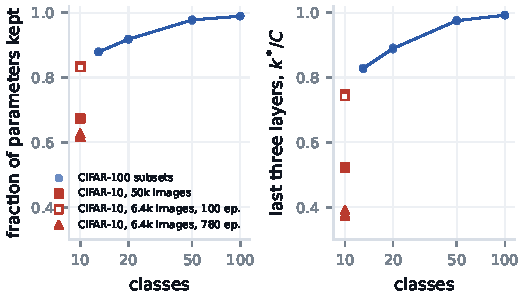
\includegraphics[width=0.92\columnwidth]{fig9_classes.pdf}
  \caption{Class count at fixed architecture and recipe (plan Section~9.12): VGG-16 (BN) on nested CIFAR-100 subsets of $13$, $20$, $50$ and $100$ classes, three seeds (dots) and their mean (line), widths read after the ReLU at $\tau = 0.999$ on each network's training images. Left: fraction of the full parameter count the ruler keeps. Right: mean $k^*(0.999)/C$ of the last three layers. Squares: the ten-class CIFAR-10 task on $50{,}000$ images (filled) and on $6{,}400$ images for the same $100$ epochs (open), the latter the image count of the thirteen-class subset; triangle: the same $6{,}400$ images for $780$ epochs, the full set's $39{,}000$ steps (plan Section~9.13).}
  \label{fig:classes}
\end{figure}

% =========================================================================
\section{Discussion}
\label{sec:discussion}

\subsection{Sources of Disagreement and Reporting Requirements}
\label{sec:why}

The reconciliation of the two published profiles is not the one we
expected. The estimator changes the level, not the ordering, by more than
the profile's own step; the summary statistic changes the ordering, in
the direction opposite to the one that would reconcile the shapes; the
tensor and the denominator each add a factor; and the terminal collapse
is the task's, present in our CIFAR-10 VGG-16 and absent in our ImageNet
one under one protocol. The two published profiles differ in what tensor
they read and what task they were trained on, and would differ in level
even if they agreed on both.

None of this is an error in any published work; each is a choice a
measurement must make, made differently without the consequence being
known.\label{sec:protocol} A reported effective-width profile should
state the tensor read (the rank bound binds the convolution output and
not the block output); whether positions or images are the observations
(the pooled value is lower at every layer by more than the step); the
denominator (the nominal width is unattainable at every expansion layer);
that depthwise and dense layers are on separate axes; the image set (on
noise the profile changes); and the sample-to-channel ratio at the widest
layer (under pooling it is the image count and fails at $2048$ channels
for any dataset under $10^5$ images). None of this is expensive: the first
measurement took about five hours on one consumer GPU and the second ran
on a laptop.

\subsection{Implications for Choosing Width}
\label{sec:implications}

Once the denominator is right, how much of its width a trained layer uses
has two answers. At the $95\%$ criterion a dense convolution uses
$0.33$--$0.72$ of its attainable rank in the median over layers across
eleven families; that number orders layers and tracks training but is not
removable width, since truncating to it costs ResNet-50 $21$ points. At
the $99.9\%$ criterion it uses $0.84$--$0.93$, and in six of eight
checkpoints truncating to that costs nothing a paired test detects. The
second number is the one a width-selection method has to explain. Read
after the nonlinearity, it is
a width a network can be built at: two thirds of VGG-16's parameters on
CIFAR-10 at full accuracy and above a uniform cut in every seed pairing,
and the full width on CIFAR-100 and ImageNet-1k, where a hundred or a
thousand classes leave no margin after the nonlinearity. Two consequences
follow for any criterion. It must read $k^*(0.999)$ after the ReLU, not
$k^*(0.95)$ at the convolution output, or it removes directions the
classifier depends on and caps what the next layer receives; and it must
divide by the attainable rank, or it reports every expansion layer as
three-quarters idle.

What differs across architectures is how much of the profile is learned.
For plain, basic-residual and dense networks the ordering is the
architecture's and training adds a level, so a criterion that sets widths
from the network at initialisation would order those layers correctly;
for the ImageNet ResNet-50 checkpoints it would not, and the controlled
experiment says the block alone is not the reason.
Whether the count can be raised by regularisation is not a matter of
pushing the kernel toward an isometry alone: the trained kernel is aligned
with its input, the decomposition predicts a rise of about $0.3\,r_{\max}$
rather than a jump to the ceiling, and the penalties in use realise half
of it, in the layers named. A width-selection method built on this
statistic is a separate piece of work; what this paper fixes is the
quantity it should optimise and the checks it must pass.

\subsection{Limitations and Failure Cases}
\label{sec:limits}

\emph{Scope of the claims.} Everything here is a linear functional of the
channel covariance at one tensor, not a manifold dimension, and a layer
whose covariance has high rank may still carry a low-dimensional manifold
(Section~\ref{sec:four}). No measurement here says by itself that a
narrower network trains to the same accuracy; where the paper says so it
is by retraining one architecture, and the statement holds for the
post-activation widths at $\tau = 0.999$ on a few-class task and nowhere
else. The paper makes two shape statements
only, the reversal of the depth trend in ResNet-50 (six recipes, five
seeds, exploratory) and the terminal collapse of few-class networks
(three seeds per class count, against its registered rule).

\emph{Where the ruler is silent or inside the noise.} The pooled
estimator cannot be read at a wide layer, and eleven of ResNet-50's
pooled rows fail our own gate. The bound $r_{\max}$ is necessary and not
sufficient: at a first layer the RGB patch sets the rank, and on
ImageNet-1k the ruler cuts the ResNet-18 stem and nothing else.
Corollary~\ref{cor:kstar} is empty when the kernel is ill-conditioned,
which at the trained median $\kappa = 10.6$ it is on about half the
layers. The pooling shift does not exceed DenseNet-121's structural step;
ConvNeXt-T's trained-versus-untrained comparison is $p = 0.013$ and
$0.21$ once its depthwise and dense layers are kept apart; and
MobileNetV3-Large's random draws agree only at $0.75$, so its reference
is itself unstable.

\emph{Registered predictions that failed.} H9.1, P9.3, P9.7, P9.10,
P9.14, P9.15, P9.21, P9.23, P9.25, P9.30, P9.32--P9.34 and the layer part
of P9.19, each reported at the place cited with its registered rule and
none softened by an unregistered re-analysis. $k^*(0.999)$ bounds the
width in use for conventional recipes and not for the RSB recipes, so the
threshold that names the width in use is recipe-dependent.

\emph{Error bars and scope.} Error bars exist for ResNet-50 (six recipes,
five seeds) and for family-level statements; the other families have one
to six checkpoints and three seeds, enough for the ordering statistics
and not for a statement about one of their layers. The controlled
experiment varies the block at CIFAR-10 scale and so cannot say whether
the ImageNet effect is the dataset's, the recipes', or theirs in
interaction with the block; the experiment that would, the same
architectures under one ImageNet recipe with seeds, is left to a study
with the compute. Head depth at fixed class count was
not varied. The inverted-residual finding is about the checkpoints one
can download. A ViT-B/16 profile against one random initialisation
(supplement, Table~S6) shows the protocol applies unchanged to linear
layers, with an ordering that is the architecture's and a level training
doubles; it is one checkpoint and one seed.

% =========================================================================
\section{Conclusion}

Two published depth profiles of how much of its width a convolutional
layer uses disagree, and they measure different objects: the denominator,
which understates every expansion layer by its expansion ratio and
misreads bottleneck networks as underused; the estimator, which lowers a
profile by about twice its own step; and the tensor, which differs by the
expansion ratio at every bottleneck block. With the choices fixed the
protocol reproduces the published CIFAR-10 table. The identity
$\Sigma_{\rm out} = W\Sigma_{\rm patch}W^{\top}$ turns the count into a
measurement of what the architecture permits, what the data supply and
what training does. Trained networks largely keep the ordering the
architecture gave them and gain a level, set by a kernel whose gain has
aligned with its input's principal directions; the ImageNet ResNet-50
checkpoints that reorder owe it to their data or recipes, alone or with
their block; and the width the ruler names after the nonlinearity can be
trained to on a few-class task, the margin it finds belonging to that
task. The same identity gives orthogonality regularisation a quantified
prediction, which the penalties in use meet by half. Code, spectra and
the pre-registered plan with its deviation log are released, so that the
next profile can be compared with these on stated terms.

% =========================================================================
\section*{Reproducibility}
\label{sec:repro}
Measurement code, analysis scripts, run manifests and the raw eigenvalue
spectra of every layer are at
\url{https://github.com/layerspec/effective-width}, with the analysis plan
and its deviation log under version control as the evidence that the
analysis was fixed before the ImageNet data were seen; every table and
figure of both documents is written by a script there from the released
spectra; the supplement
holds the proofs, the claims table with the status of every registered
prediction, and the secondary tables and figures. The measurement is
packaged: \texttt{pip install layerspec} gives
\texttt{layerspec.profile(model, loader)} and
\texttt{layerspec.decompose(model, loader)} for any PyTorch network with
convolutional or linear layers.
\todo{repository is private until submission; make public and add the release tag here.}

\bibliographystyle{IEEEtran}
\bibliography{refs}

\end{document}
